\documentclass[10pt]{article}
\usepackage{listings}
\usepackage{graphicx}
\usepackage{verbatim}
\begin{document}
\title{CS 378: Programming For Performance Project 3}
\author{Sai Avala \\ Vaibhav Gupta \\ Sudheesh Katkam}
\date{November 10, 2014}
\maketitle
\section{Introduction}
\label{introduction}
\sf For this project we parallelized Dijkstra's Single Source Shortest Path (SSSP) algorithm and tested this
function against the full US Road Map Travel Graph. We implemented four separate schedulers to show the variations
in performance when applied to the parallelized Dijkstra's algorithm. These four schedulers are as follows:
\begin{itemize}
    \item Global LIFO
    \item Global FIFO
    \item Global Priority Queue
    \item Priority queue per thread, work is pushed locally, threads steal when out of work
\end{itemize}

\section{Dijkstras Algorithm}
\label{dijkstrasAlgoritm}
\sf Dijkstras algorithm is a graph search algorithm solves for the shortest path from a single source
given non-negative edge weights. Essentially what this algorithm does is that given a starting node,
it will go ahead, pick the rest of the neighbors, calculates the difference between the current
node and the neighboring nodes and updates the distances for each neighboring node if it
is smaller. 

\newpage \section{Results}
\label{results}
\sf This section here displays both the results and plots for the different schedulers. By looking
at the graphs on the subsequen pages, we notice that our FIFO Queue scheudler implementation works
the best. There are points in the graph where the data might seem "random". However, this could 
possibly be explained by the fact that the total run time for the whole data set is not that long.
Then, when generating threads to work with the small runtime, we would run into seemingly random 
results because the generation of threads and joining of the threads could change the actual time.
What we noticed here is that unless the working set size is somewhat large, generating threads
would seem to provide soemwhat unusual results. Also, please note that we ran this project on the
NYC Travel Time graph, not the Full USA graph. This is because runtimes for LIFO would have been
over 7+ hours, and there wasn't enough Service Units allocation available on Stampede to actually
run the program.
\newline The raw data results are below:
\begin{verbatim}
    32 Threads
./project3 32 nyc-raod.gr 733846
----Queue----
Time:   0.000054
----Stack----
Time:   0.000051
----Priority Queue----
Time:   0.000056
----Shared Priority Queue----
Time:   0.000050

    16 Threads
./project3 16 nyc-raod.gr 366923
----Queue----
Time:   0.000008
----Stack----
Time:   0.000027
----Priority Queue----
Time:   0.000012
----Shared Priority Queue----
Time:   0.000016

    8 Threads
./project3 8 nyc-raod.gr 183462
----Queue----
Time:   0.000006
----Stack----
Time:   0.000047
----Priority Queue----
Time:   0.000062
----Shared Priority Queue----
Time:   0.000064

    4 Threads
./project3 4 nyc-raod.gr 91731
----Queue----
Time:   0.000037
----Stack----
Time:   0.000021
----Priority Queue----
Time:   0.000052
----Shared Priority Queue----
Time:   0.000112

    2 Threads
./project3 2 nyc-raod.gr 45866
----Queue----
Time:   0.000052
----Stack----
Time:   0.000087
----Priority Queue----
Time:   0.000041
----Shared Priority Queue----
Time:   0.000050

    1 Thread
./project3 1 nyc-raod.gr 22933
----Queue----
Time:   0.000046
----Stack----
Time:   0.000017
----Priority Queue----
Time:   0.000056
----Shared Priority Queue----
Time:   0.000050

\end{verbatim}
\subsection{Queue Scheduler Results}
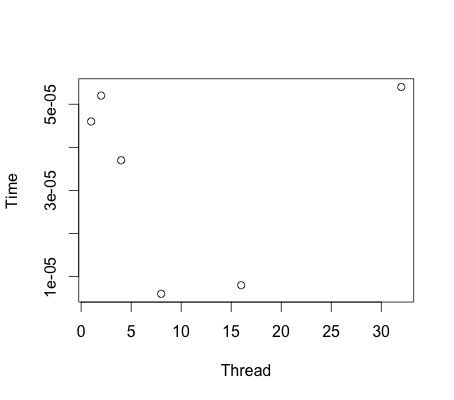
\includegraphics[width=1.0\textwidth]{queue.png}

\subsection{Stack Scheduler Results}
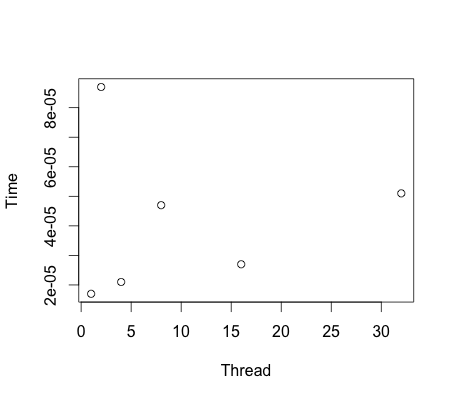
\includegraphics[width=1.0\textwidth]{stack.png}

\subsection{Global Priority Queue Scheduler Results}
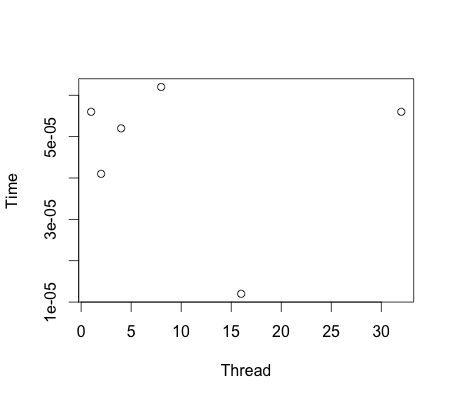
\includegraphics[width=1.0\textwidth]{priorityQueue.png}

\subsection{Shared Priority Queue Scheduler Results}
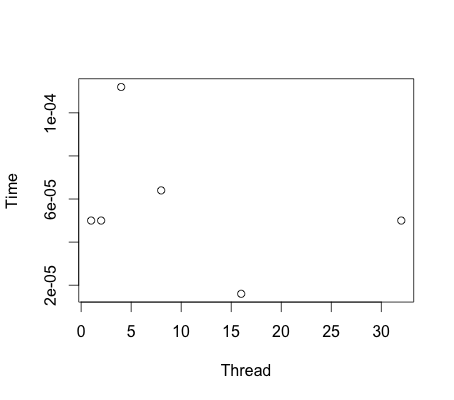
\includegraphics[width=1.0\textwidth]{sharedPriorityQueue.png}


\begin{comment}
\subsection{Plots}
\pagebreak \includegraphics[width=1.0\textwidth]{PAPI-LST-INS.png}
\pagebreak \includegraphics[width=1.0\textwidth]{PAPI-FP-INS.png}
\includegraphics[width=1.0\textwidth]{PAPI-L1-DCM.png}
\pagebreak \includegraphics[width=1.0\textwidth]{PAPI-L2-TCM.png}
\end{comment}


\end{document}
